\documentclass[conference,a4paper]{IEEEtran}
\IEEEoverridecommandlockouts
\usepackage[utf8]{inputenc}
\usepackage[T1]{fontenc}
\usepackage[spanish,es-tabla,es-noshorthands,es-nodecimaldot]{babel}
\usepackage{amsmath,amssymb}
\usepackage{graphicx}
\usepackage{booktabs}
\usepackage{multirow}
\usepackage{array}
\usepackage{cite}
\usepackage{microtype}
\usepackage{xcolor}
\usepackage{tikz}
\usetikzlibrary{positioning,arrows.meta,fit}
\usepackage[hidelinks]{hyperref}
\graphicspath{{figuras/}{../figuras/}}
\newcolumntype{L}[1]{>{\raggedright\arraybackslash}p{#1}}
\renewcommand{\arraystretch}{1.12}

\begin{document}

\title{Predicción del tiempo de llegada entre puntos de control en una ruta de transporte urbano del Cusco mediante aprendizaje automático\\[4pt]
\large Entregable 2: implementación y evaluación experimental}

\author{\IEEEauthorblockN{Divano Estefano Perez Nina, Ángel Fredy Cerdan Cigüeñas,\\Alfredo Ernesto Sanchez Tuesta, Renzo Kei Shimabukuro Kohatsu}
\IEEEauthorblockA{Curso 1INF02 Aprendizaje de Máquina, semestre 2026-2\\
Pontificia Universidad Católica del Perú, Lima, Perú}}

\maketitle

\begin{abstract}
En el transporte urbano del Cusco los buses deben pasar por puntos de control a horas programadas, pero estos horarios son fijos y no reflejan cómo cambia el tráfico durante el día. Este trabajo predice, cuando un bus pasa por un punto de control, cuánto tardará en llegar a cualquier punto posterior de su ruta. Se usaron los registros de paso por los dieciocho puntos de control y la posición satelital de cuarenta y cinco buses durante un mes, complementados con datos meteorológicos y de altitud. Se entrenó un único modelo de regresión para todos los trayectos y se compararon ocho algoritmos supervisados con tres referencias sin aprendizaje: el horario, el promedio histórico y el último bus que hizo el mismo trayecto. Con una partición temporal, Random Forest obtuvo el menor error, con 1,90 minutos de error absoluto medio frente a 2,40 minutos del promedio histórico, una reducción de 20,8 por ciento que confirma la hipótesis planteada. La ventaja crece con la distancia entre los puntos y se explica sobre todo por el estado del bus y por los buses que acaban de recorrer el trayecto, mientras que el clima no aporta e incluso empeora la predicción. Además, la regresión cuantílica entrega un rango de llegada que contiene al valor real en tres de cada cuatro casos, algo menos de lo esperado.
\end{abstract}

\begin{IEEEkeywords}
tiempo de llegada, transporte público, aprendizaje automático, regresión, regresión cuantílica, Cusco
\end{IEEEkeywords}

% =====================================================================
\section{Introducción}

\subsection{Contexto}
El Cusco concentra en un centro histórico de vías estrechas la mayor parte de los recorridos de transporte urbano: el Plan Cusco al 2025 estima que el 90\,\% de las rutas pasan necesariamente por el centro, lo que genera competencia por el espacio vial, mientras que cerca del 39\,\% de los desplazamientos se realiza en transporte público~\cite{concha2018}. En una encuesta a 384 usuarios, el 76,1\,\% calificó la calidad del servicio de transporte urbano como regular, y se reportó hacinamiento frecuente en las unidades~\cite{delgado2021}.

La operación de las rutas se controla mediante \emph{puntos de control}: cada vuelta tiene una hora programada de paso por cada punto, y las desviaciones se registran para supervisar a los conductores. El conjunto de datos de este proyecto proviene de un sistema de transporte inteligente (STI) que registra, para una ruta del Cusco, la hora programada y la hora real de paso por 18 puntos de control, junto con la posición GPS de cada bus cada pocos segundos.

\subsection{Problema}
Los horarios programados son estáticos. En la ruta analizada el operador utiliza solo cuatro plantillas de horario, con duraciones de vuelta de 147, 161, 168 y 170~min, para cubrir 16 horas de operación y los siete días de la semana. Sin embargo, el tiempo real de cada tramo cambia con la hora del día y las condiciones del tráfico: los buses tienden a adelantarse en la madrugada (desviación media de $-1{,}2$~min por tramo a las 5:00) y a retrasarse por la tarde ($+0{,}9$~min entre las 18:00 y las 19:00).

Esto tiene dos consecuencias. Para el \emph{operador}, el horario no permite distinguir los retrasos causados por el tráfico de los causados por la conducción, y empuja a los conductores a acelerar o a detenerse para cumplirlo. Para el \emph{usuario}, no existe información confiable sobre cuánto tardará su viaje. Los datos que permitirían estimarlo ya existen, pero solo se usan para el control y la sanción.

\subsection{Pregunta de investigación e hipótesis}
\textbf{Pregunta.} ¿Puede un modelo de aprendizaje automático estimar el tiempo de llegada de un bus entre dos puntos de control cualesquiera con mayor precisión que el horario programado, el promedio histórico y el tiempo del último bus?

\textbf{Hipótesis.} En la predicción del tiempo de llegada de A a B, el mejor modelo reduce el error absoluto medio (MAE) global en al menos 15\,\% frente a la mejor referencia sin aprendizaje.

\subsection{Objetivos}
\textbf{Objetivo general.} Desarrollar y evaluar modelos de aprendizaje automático que estimen el tiempo de llegada de un bus entre dos puntos de control de una ruta urbana del Cusco, y presentarlos en una demostración interactiva.

\textbf{Objetivos específicos.}
\begin{enumerate}
\item Construir un conjunto de datos de trayectos A$\to$B a partir de los registros de puntos de control y GPS, con limpieza y detección de anomalías.
\item Comparar ocho algoritmos de regresión frente a tres referencias sin aprendizaje mediante un diseño experimental con partición temporal.
\item Analizar cómo varía el error con la distancia entre A y B y qué grupos de variables aportan a la predicción.
\item Estimar intervalos de predicción (percentiles 10--90) y evaluar su cobertura.
\end{enumerate}

\textbf{Cambio de alcance respecto al Entregable 1.} La propuesta incluía técnicas de clustering (DBSCAN para ubicar paraderos; K-Means, Ward y mezclas gaussianas para identificar regímenes de tráfico). Siguiendo la recomendación de los docentes de concentrar el proyecto en un solo tipo de tarea, se optó por la regresión, que responde directamente a la pregunta de investigación. Por ello se retiran el clustering de regímenes y las variables derivadas de DBSCAN, cuyo aporte a la predicción fue además despreciable en una evaluación preliminar (MAE de 0,850 frente a 0,851~min con y sin ellas). Se mantienen Isolation Forest para la limpieza de datos y PCA como experimento de reducción de dimensionalidad.

% =====================================================================
\section{Trabajos relacionados}\label{sec:rel}

\subsection{Predicción del tiempo de llegada de buses}
La predicción del tiempo de llegada (ETA) de buses se ha abordado con redes neuronales artificiales desde inicios de los 2000~\cite{chien2002} y con máquinas de vectores de soporte~\cite{bin2006}. Yu \emph{et~al.}~\cite{yu2011} compararon SVM, redes neuronales, $k$ vecinos más cercanos y regresión lineal para predecir la llegada a un paradero compartido por varias rutas; el SVM obtuvo el mejor desempeño y los modelos que usaban información de varias rutas superaron a los de una sola. Más recientemente, Petersen \emph{et~al.}~\cite{petersen2019} propusieron una red convolucional LSTM que predice simultáneamente los tiempos de todos los enlaces de una ruta de Copenhague varios pasos adelante, y superó al promedio histórico y al modelo en producción del operador, sobre todo en hora punta. Rodríguez-Deniz y Villani~\cite{rodriguez2022} plantearon un modelo bayesiano con errores $t$ de Student para manejar retrasos de cola pesada, que combina variables de buses anteriores para el corto plazo con procesos gaussianos para horizontes largos.

En su revisión de 40 estudios, Reich \emph{et~al.}~\cite{reich2019} encontraron que la diversidad de métricas y la frecuente omisión de comparaciones con referencias simples impiden comparar objetivamente los métodos, y recomendaron publicar referencias y código. Este trabajo adopta esa recomendación: todos los modelos se comparan con tres referencias sin aprendizaje y el código es reproducible.

\subsection{Incertidumbre en la predicción}
Una predicción puntual no indica cuánto confiar en ella. Petersen \emph{et~al.}~\cite{petersen2021} compararon la regresión cuantílica profunda y las redes recurrentes bayesianas para aproximar la distribución del tiempo de viaje hasta un punto de transbordo. La regresión cuantílica~\cite{koenker1978} permite estimar directamente percentiles de la variable objetivo y puede combinarse con métodos de \emph{boosting}~\cite{friedman2001}.

\subsection{Variabilidad del tiempo de viaje y variables externas}
Mazloumi \emph{et~al.}~\cite{mazloumi2010} usaron datos GPS para analizar la variabilidad del tiempo de viaje del transporte público y sus factores. Para detectar registros anómalos, Isolation Forest~\cite{liu2008} aísla las observaciones atípicas sin necesidad de etiquetas. En cuanto a variables externas, Tsapakis \emph{et~al.}~\cite{tsapakis2013} cuantificaron el aumento de los tiempos de viaje urbanos con la lluvia y la nieve.

\subsection{Brecha}
La Tabla~\ref{tab:rel} resume los trabajos más cercanos. La mayoría predice el tiempo al siguiente paradero o por enlace, en ciudades con redes extensas y abundantes datos. Este proyecto se diferencia en dos aspectos: (i) predice con un único modelo el tiempo a cualquier punto posterior de la ruta, con un rango de incertidumbre; y (ii) se aplica a un sistema de puntos de control en una ciudad intermedia andina, con un mes de datos.

\begin{table}[t]
\centering
\caption{Trabajos relacionados más cercanos}
\label{tab:rel}
\footnotesize
\begin{tabular}{@{}L{1.25cm}L{2.0cm}L{2.0cm}L{1.95cm}@{}}
\toprule
Trabajo & Datos & Método & Salida \\
\midrule
\cite{yu2011} & Encuestas de campo, varias rutas & SVM, RNA, $k$NN, RL & Llegada a un paradero \\
\cite{petersen2019} & AVL, Copenhague & ConvLSTM & Tiempos de todos los enlaces \\
\cite{rodriguez2022} & Buses urbanos de alta frecuencia & Bayesiano, $t$ de Student, PG & Retraso en tiempo real \\
\cite{petersen2021} & AVL & Cuantiles profundos, RNN bayesiana & Distribución del tiempo de viaje \\
\midrule
Este trabajo & Puntos de control y GPS, Cusco & 8 regresores, regresión cuantílica & ETA A$\to$B con intervalo \\
\bottomrule
\end{tabular}
\end{table}

% =====================================================================
\section{Conjunto de datos y análisis exploratorio}\label{sec:data}

Los datos fueron proporcionados por los docentes y provienen de un STI de una ruta de transporte urbano del Cusco. Constan de dos archivos (Tabla~\ref{tab:data}).

\begin{table}[t]
\centering
\caption{Archivos del conjunto de datos}
\label{tab:data}
\footnotesize
\begin{tabular}{@{}L{2.15cm}L{5.65cm}@{}}
\toprule
Archivo & Contenido \\
\midrule
\texttt{Times.csv} & 4\,707 vueltas de 45 buses (6 de enero al 1 de febrero de 2025, 27 días). Columnas: \texttt{id}, \texttt{lap} (vuelta del día, 1--8), \texttt{date}, \texttt{time} (salida programada), \texttt{start\_time} (arreglo de 18 horas programadas), \texttt{end\_time} (arreglo de 18 horas reales), \texttt{difference\_time} (arreglo de 18 desviaciones en minutos) y \texttt{vehicle\_id\_id}. \\
\addlinespace
\texttt{Monitoring.csv} & 1\,630\,431 registros GPS de los mismos 45 buses (1 de enero al 1 de febrero de 2025). Columnas: \texttt{id}, \texttt{date}, \texttt{time}, \texttt{lap} (0 = fuera de vuelta), \texttt{latitude}, \texttt{longitude}, \texttt{speed} (km/h), \texttt{bearing} (rumbo en grados) y \texttt{vehicle\_id\_id}. \\
\bottomrule
\end{tabular}
\end{table}

\textbf{Estructura de la ruta.} Todas las vueltas recorren la misma ruta circular con 18 puntos de control (Fig.~\ref{fig:ruta}). La ubicación de cada punto no está en los datos; se estimó como la mediana de la posición GPS del bus en el instante de paso. A diferencia de lo que indica la documentación original, \texttt{start\_time}, \texttt{end\_time} y \texttt{difference\_time} no son valores únicos sino arreglos de 18 elementos, uno por punto de control. Al expandirlos se obtienen 84\,726 pasos por punto de control, de los cuales 7\,746 (9,1\,\%) no fueron registrados (hora real \texttt{00:00:00}).

\begin{figure}[t]
\centering
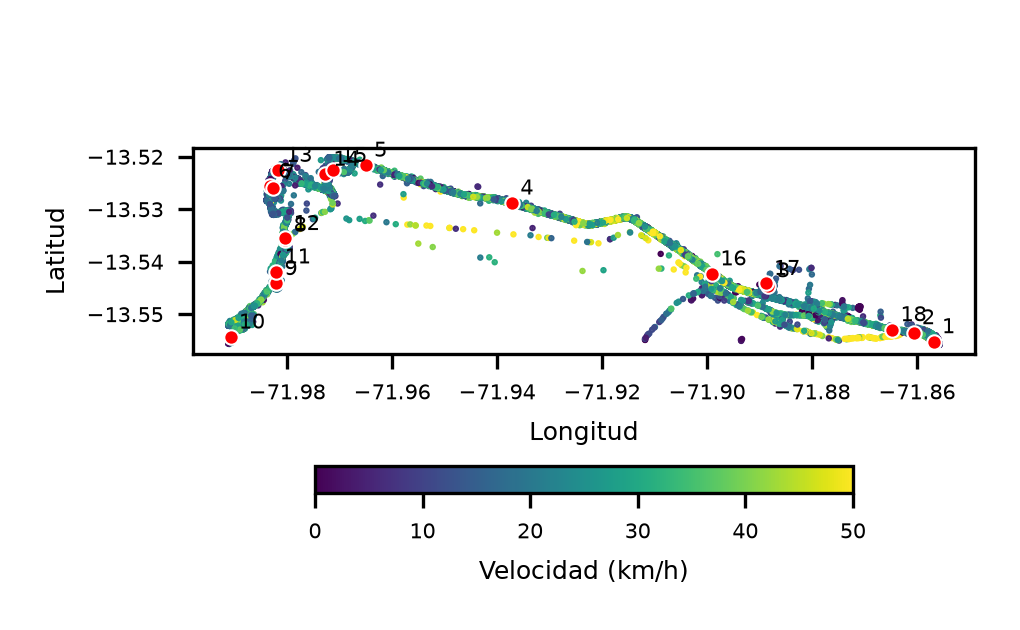
\includegraphics[width=\columnwidth, trim=0 0 0 27, clip]{fig1_ruta.png}
\caption{Registros GPS coloreados por velocidad y ubicación estimada de los 18 puntos de control de la ruta.}
\label{fig:ruta}
\end{figure}

\textbf{Horario frente a tiempos reales.} La duración mediana de la vuelta es de 164~min frente a 161~min programados, con un rango de 148 a 179~min entre los percentiles 10 y 90. Los tramos duran en promedio 9,7~min, aunque varían entre menos de 1 y cerca de 30~min (Fig.~\ref{fig:tramos}). Usado como predicción, el horario tiene un error absoluto medio de 1,56~min por tramo, con tramos críticos como el 13$\to$14 (3,2~min).

\begin{figure}[t]
\centering
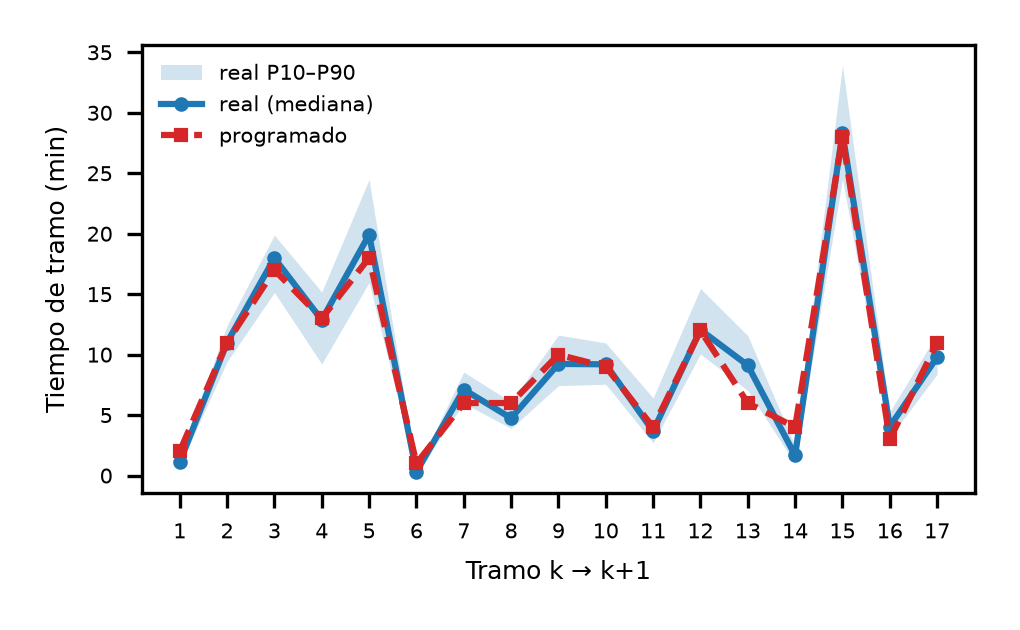
\includegraphics[width=\columnwidth]{fig2_tramos.png}
\caption{Tiempo programado y tiempo real (mediana y banda P10--P90) de cada tramo de la ruta.}
\label{fig:tramos}
\end{figure}

\textbf{Datos externos.} Se consultó la API de Open-Meteo con las coordenadas de cada uno de los 18 puntos de control: la altitud (modelo de elevación de 90~m; entre 3\,185 y 3\,519~m) y el clima horario del reanálisis ERA5~\cite{hersbach2020} (temperatura, humedad, precipitación, nubosidad y viento), corrigiendo la temperatura por la altitud de cada punto. La grilla del reanálisis tiene unos 7~km, por lo que los 18 puntos comparten dos celdas de precipitación, a 3~km de distancia en promedio. Enero es temporada de lluvias (47\,\% de las horas con precipitación), pero la desviación media frente al horario solo pasa de $+0{,}24$~min por tramo en horas secas a $+0{,}35$~min con lluvia mayor a 1~mm.

% =====================================================================
\section{Metodología}\label{sec:met}

La Fig.~\ref{fig:pipeline} resume la metodología.

\begin{figure}[t]
\centering
\begin{tikzpicture}[
  node distance=3.5mm and 3mm,
  box/.style={draw, rounded corners=2pt, align=center, font=\scriptsize, minimum height=7mm, inner sep=2pt},
  data/.style={box, fill=gray!12},
  sup/.style={box, fill=blue!10},
  uns/.style={box, fill=orange!15},
  arr/.style={-{Stealth[length=2mm]}, thick}]
\node[data, text width=1.55cm] (t) {Times.csv\\(puntos de control)};
\node[data, text width=1.55cm, right=of t] (m) {Monitoring.csv\\(GPS)};
\node[data, text width=1.55cm, right=of m] (c) {Open-Meteo\\(clima, altitud)};
\node[uns, text width=7.0cm, below=of m] (pre) {Preprocesamiento: limpieza, Isolation Forest, imputación para el \emph{headway}, ubicación de puntos de control};
\node[box, text width=7.0cm, below=of pre] (feat) {Dataset de trayectos A$\to$B: un ejemplo por paso $(i,k)$ y destino $k{+}\Delta$, variables conocidas en $a_{i,k}$};
\node[sup, text width=7.0cm, below=of feat] (mod) {Regresión A$\to$B: 8 modelos y regresión cuantílica (P10, P50, P90)};
\node[box, text width=7.0cm, below=of mod] (eval) {Evaluación: partición temporal, 3 referencias, MAE, WAPE, P90, Wilcoxon, cobertura};
\node[box, text width=7.0cm, below=of eval, fill=green!10] (demo) {Demostración interactiva};
\draw[arr] (t) -- (t |- pre.north); \draw[arr] (m) -- (pre); \draw[arr] (c) -- (c |- pre.north);
\draw[arr] (pre) -- (feat); \draw[arr] (feat) -- (mod); \draw[arr] (mod) -- (eval); \draw[arr] (eval) -- (demo);
\end{tikzpicture}
\caption{Metodología. En naranja, preprocesamiento con técnicas no supervisadas; en azul, modelos supervisados.}
\label{fig:pipeline}
\end{figure}

\subsection{Formulación del problema}
Sea $a_{i,k}$ la hora real de paso de la vuelta $i$ por el punto $k$ y $s_{i,k}$ la hora programada. Para cada paso registrado y cada destino $k+\Delta$, con $\Delta \in \{1,\dots,17\}$ y $k+\Delta \le 18$, la variable objetivo es
\begin{equation}
y_{i,k,\Delta} = a_{i,k+\Delta} - a_{i,k} \quad \text{(minutos)},
\end{equation}
y el modelo debe estimarla usando solo información disponible en el instante $a_{i,k}$. Se entrena un único modelo para todos los pares A$\to$B, con $\Delta$ como variable de entrada. Esta formulación responde a la pregunta del usuario (``¿cuándo llego a mi destino?'') en lugar de limitarse al siguiente punto.

\subsection{Preprocesamiento}
\begin{itemize}
\item \textbf{Limpieza de pasos:} se descartan los pasos no registrados (7\,746), las desviaciones mayores a 60~min (156) y las horas reales no monotónicas dentro de una vuelta (ninguna).
\item \textbf{Anomalías:} Isolation Forest~\cite{liu2008}, ajustado solo con los días de entrenamiento, sobre el retraso y su variación en el último tramo (contaminación 0,1\,\%; 88 pasos marcados) y sobre posición y velocidad en el GPS (0,5\,\%; 8\,180 registros marcados, además de 6\,783 duplicados). Quedan 76\,736 pasos válidos.
\item \textbf{Imputación:} los retrasos faltantes se interpolan dentro de la vuelta (máximo dos puntos seguidos) solo para calcular el intervalo con el bus de adelante (\emph{headway}); nunca se usan como objetivo.
\item \textbf{GPS por tramo:} cada registro GPS se asigna al tramo que termina en el siguiente paso del mismo vehículo; por tramo se calcula la velocidad media y la fracción de registros a 5~km/h o menos (el equipo casi no registra velocidad 0).
\end{itemize}
El resultado son 622\,845 trayectos A$\to$B.

\subsection{Variables}
La Tabla~\ref{tab:vars} agrupa las variables. Todas se calculan con información anterior a $a_{i,k}$: por ejemplo, el ``último bus'' es el que terminó el mismo trayecto A$\to$B antes de ese instante, y si lo hizo hace más de 60~min se considera que ya no informa del tráfico actual.

\begin{table}[t]
\centering
\caption{Grupos de variables de entrada}
\label{tab:vars}
\footnotesize
\begin{tabular}{@{}L{1.7cm}L{6.1cm}@{}}
\toprule
Grupo & Variables \\
\midrule
Estado del bus & retraso en A, variación del retraso en el último tramo, duración del último tramo, \emph{headway}, número de vuelta \\
Buses recientes & tiempo del último bus en el mismo trayecto, media de los tres últimos, antigüedad de esa información \\
GPS & velocidad media y fracción detenida del bus (último tramo) y del último bus (primer tramo del trayecto) \\
Clima & temperatura, humedad, precipitación (1 y 3~h), nubosidad, viento en A a la hora del paso \\
Altitud & altitud de A y desnivel entre A y B \\
Contexto & origen $k$, distancia $\Delta$, hora, día de la semana, tiempo programado de A a B, vehículo \\
\bottomrule
\end{tabular}
\end{table}

\subsection{Algoritmos y justificación}
Se evaluaron ocho algoritmos de \texttt{scikit-learn}~\cite{pedregosa2011} que cubren familias distintas, para no depender de un único supuesto sobre la relación entre las variables y el tiempo de viaje (Tabla~\ref{tab:alg}). Todos comparten un mismo \emph{pipeline}: imputación por mediana y estandarización de las variables numéricas, y codificación \emph{one-hot} del vehículo.

\begin{table}[t]
\centering
\caption{Algoritmos de regresión y justificación}
\label{tab:alg}
\footnotesize
\begin{tabular}{@{}L{1.55cm}L{6.25cm}@{}}
\toprule
Algoritmo & Justificación \\
\midrule
Ridge & Referencia lineal regularizada; interpretable y de bajo costo. \\
$k$NN & No paramétrico; predice con viajes similares del historial~\cite{yu2011}. \\
Árbol de decisión & Captura interacciones (tramo $\times$ hora) con reglas interpretables. \\
SVM (RBF) & Buen desempeño en estudios previos de ETA~\cite{bin2006,yu2011}. \\
Random Forest & Ensamble por \emph{bagging}~\cite{breiman2001}; robusto al ruido y a variables poco informativas. \\
AdaBoost & Ensamble secuencial que enfatiza los casos difíciles. \\
Gradient Boosting & \emph{Boosting} por gradiente~\cite{friedman2001} (\texttt{HistGradientBoosting}); maneja valores faltantes y admite pérdida cuantílica. \\
MLP & Red neuronal, representativa de los enfoques con redes~\cite{chien2002}. \\
\bottomrule
\end{tabular}
\end{table}

\subsection{Intervalos de predicción}
Se entrenó Gradient Boosting con la pérdida cuantílica~\cite{koenker1978}
\begin{equation}
L_\tau(y,\hat{y}) = \max\big(\tau\,(y-\hat{y}),\,(\tau-1)\,(y-\hat{y})\big)
\end{equation}
para $\tau \in \{0{,}1;\,0{,}5;\,0{,}9\}$, con los hiperparámetros elegidos para la predicción puntual, de modo que cada predicción venga acompañada de un rango P10--P90.

% =====================================================================
\section{Experimentación y resultados}\label{sec:exp}

\subsection{Setup experimental}
\textbf{Validación.} Como los datos son series temporales, una partición aleatoria mezclaría viajes del mismo día entre entrenamiento y prueba y sobrestimaría el desempeño~\cite{bergmeir2012}. Se usó una partición temporal por días: entrenamiento del 6 al 22 de enero (386\,332 ejemplos), validación del 23 al 26 de enero (88\,646) y prueba del 27 de enero al 1 de febrero (147\,867).

\textbf{Ajuste de hiperparámetros.} Para cada algoritmo se evaluaron seis combinaciones elegidas al azar del espacio de la Tabla~\ref{tab:hpgrid}, entrenando con una submuestra de 60\,000 ejemplos y midiendo el MAE en validación. Con la mejor combinación (Tabla~\ref{tab:hp}) el modelo se reentrenó con entrenamiento y validación y se evaluó una sola vez en prueba. Por su costo, SVM se entrenó con una submuestra de 8\,000 ejemplos y $k$NN, AdaBoost y MLP con 150\,000. La semilla aleatoria es 42.

\begin{table}[t]
\centering
\caption{Espacio de búsqueda de hiperparámetros}
\label{tab:hpgrid}
\footnotesize
\begin{tabular}{@{}L{1.7cm}L{6.1cm}@{}}
\toprule
Modelo & Valores explorados \\
\midrule
Ridge & $\alpha \in \{0{,}01;\,0{,}1;\,1;\,10;\,100\}$ \\
$k$NN & $k \in \{5, 15, 51\}$; pesos uniformes o por distancia \\
Árbol & profundidad $\in \{5, 10, 20\}$; mín. por hoja $\in \{1, 20, 100\}$ \\
SVM & $C \in \{0{,}1;\,1;\,10\}$; $\gamma \in \{0{,}01;\,0{,}1;\,\text{scale}\}$ \\
Random Forest & árboles $\in \{200, 500\}$; profundidad $\in \{10, 20, \text{sin límite}\}$; mín. por hoja $\in \{1, 5, 20\}$ \\
AdaBoost & estimadores $\in \{100, 300\}$; tasa $\in \{0{,}1;\,1\}$; árboles de profundidad 4 \\
Gradient Boosting & tasa $\in \{0{,}03;\,0{,}1\}$; profundidad $\in \{4, 6, 8\}$; hasta 1\,000 iteraciones con parada temprana \\
MLP & capas $\in \{(64,32), (128,64,32)\}$; $\alpha \in \{10^{-4}, 10^{-3}\}$; tasa $\in \{10^{-3}, 10^{-4}\}$ \\
\bottomrule
\end{tabular}
\end{table}

\begin{table}[t]
\centering
\caption{Hiperparámetros elegidos en validación}
\label{tab:hp}
\footnotesize
\begin{tabular}{@{}L{1.7cm}L{6.1cm}@{}}
\toprule
Modelo & Hiperparámetros \\
\midrule
Ridge & \texttt{alpha}=100 \\
$k$NN & \texttt{weights}=distance, \texttt{n\_neighbors}=15 \\
Árbol de decisión & \texttt{min\_samples\_leaf}=20, \texttt{max\_depth}=20 \\
SVM (RBF) & \texttt{gamma}=scale, \texttt{C}=10 \\
Random Forest & \texttt{n\_estimators}=200, \texttt{min\_samples\_leaf}=5, \texttt{max\_depth}=20 \\
AdaBoost & \texttt{n\_estimators}=100, \texttt{learning\_rate}=0.1 \\
Gradient Boosting & \texttt{max\_depth}=6, \texttt{learning\_rate}=0.1 \\
MLP & \texttt{learning\_rate\_init}=0.001, \texttt{hidden\_layer\_sizes}=(64, 32), \texttt{alpha}=0.001 \\
\bottomrule
\end{tabular}
\end{table}

\textbf{Referencias sin aprendizaje.} (i) \emph{Horario}: $\hat{y} = s_{i,k+\Delta} - s_{i,k}$; (ii) \emph{histórico}: tiempo medio de A a B en entrenamiento y validación para el mismo origen, $\Delta$ y hora; (iii) \emph{último bus}: tiempo del último bus que completó el mismo trayecto antes de $a_{i,k}$, o el horario si no hay uno reciente.

\textbf{Métricas.} Con $e_j = y_j - \hat{y}_j$ y $n$ ejemplos de prueba:
\begin{gather}
\text{MAE} = \tfrac{1}{n}\textstyle\sum_j |e_j|, \qquad
\text{RMSE} = \sqrt{\tfrac{1}{n}\textstyle\sum_j e_j^2},\\
\text{WAPE} = \frac{\sum_j |e_j|}{\sum_j y_j}, \qquad
\text{Mejora} = 1 - \frac{\text{MAE}_{\text{modelo}}}{\text{MAE}_{\text{mejor ref.}}}.
\end{gather}
Se reportan además el porcentaje de predicciones con $|e_j| \le 2$~min y el percentil 90 de $|e_j|$ (P90). El MAE es la métrica principal. No se usa el MAPE porque se vuelve inestable cuando el valor real es pequeño~\cite{hyndman2006}, como en los tramos de 1--2~min de esta ruta, ni el $R^2$, porque el tiempo de viaje depende sobre todo de $\Delta$ y un predictor trivial ya alcanza valores altos. Para los intervalos se mide la \emph{cobertura}: el porcentaje de valores reales dentro del rango P10--P90 (ideal: 80\,\%).

\textbf{Experimentos.} E1: comparación de los ocho modelos y las tres referencias en todos los pares A$\to$B. E2: error según la distancia $\Delta$. E3: ablación por grupos de variables con Gradient Boosting. E4: efecto de PCA (95\,\% de la varianza) en $k$NN y SVM. E5: sensibilidad a hiperparámetros y costo computacional. E6: análisis del error por origen y hora, y prueba de Wilcoxon de rangos con signo (unilateral) sobre el MAE por bloques día $\times$ origen $\times$ $\Delta$~\cite{demsar2006}. E7: cobertura y ancho del intervalo P10--P90.

\textbf{Entorno computacional.} Python 3.14.0, scikit-learn 1.9.1, pandas 3.0.2, NumPy 2.4.2 y SciPy 1.18.0, en Windows 11 con 16 núcleos lógicos y 15.2 GB de RAM. La ejecución completa del cuaderno toma unos 118~min.

\subsection{Resultados y discusión}

\textbf{E1: comparación de modelos.} La Tabla~\ref{tab:e1} y la Fig.~\ref{fig:e1} muestran el desempeño en prueba. Random Forest obtuvo el menor MAE (1,90~min), seguido de cerca por Gradient Boosting (1,92~min), que entrena con un costo mucho menor (58~s frente a 4\,202~s). Frente a la mejor referencia, el promedio histórico (2,40~min), la reducción del MAE es de \textbf{20,8\,\%}, por lo que \textbf{la hipótesis se confirma}; frente al horario la reducción es de 43\,\%. El modelo acierta con un margen de $\pm 2$~min en el 66\,\% de los casos (59\,\% el histórico) y su error relativo es de 3,3\,\% del tiempo total de viaje. Los ensambles de árboles, el árbol de decisión y la MLP superan al histórico porque combinan el patrón por tramo y hora con la información del día; Ridge no lo logra porque la relación entre las variables y el tiempo de viaje no es lineal. $k$NN, SVM y AdaBoost tienen incluso más error que el horario: $k$NN y SVM dependen de distancias en un espacio de 70 dimensiones donde $\Delta$ y el tiempo programado dominan, SVM solo pudo entrenarse con 8\,000 ejemplos, y AdaBoost con árboles poco profundos no captura las interacciones entre origen, distancia y hora. La referencia del último bus es la peor porque, para trayectos largos, ese bus partió mucho antes y refleja condiciones ya pasadas.

\begin{table}[t]
\centering
\caption{E1: desempeño en prueba (todos los pares A$\to$B)}
\label{tab:e1}
\footnotesize
\setlength{\tabcolsep}{3.5pt}
\begin{tabular}{@{}lrrrrrr@{}}
\toprule
Modelo & MAE & RMSE & WAPE & $\le$2\,min & P90 & Entren. \\
 & (min) & (min) & (\%) & (\%) & (min) & (s) \\
\midrule
Ref. histórico & 2,40 & 3,67 & 4,1 & 59,1 & 5,33 & -- \\
Ref. horario & 3,34 & 5,05 & 5,7 & 48,2 & 7,83 & -- \\
Ref. último bus & 3,92 & 6,17 & 6,7 & 44,5 & 9,33 & -- \\
\midrule
\textbf{Random Forest} & \textbf{1,90} & \textbf{2,79} & \textbf{3,3} & \textbf{66,3} & \textbf{4,33} & \textbf{4\,202} \\
Gradient Boosting & 1,92 & 2,77 & 3,3 & 65,4 & 4,23 & 58 \\
Árbol de decisión & 2,19 & 3,24 & 3,7 & 61,7 & 5,03 & 10 \\
MLP & 2,28 & 3,24 & 3,9 & 58,1 & 4,97 & 32 \\
Ridge & 2,85 & 3,99 & 4,9 & 48,6 & 6,22 & 2 \\
SVM (RBF) & 3,67 & 6,33 & 6,3 & 44,2 & 7,74 & 9 \\
AdaBoost & 3,80 & 4,97 & 6,5 & 34,7 & 7,94 & 161 \\
$k$NN & 4,59 & 6,19 & 7,9 & 28,9 & 9,45 & 0 \\
\bottomrule
\end{tabular}
\end{table}

\begin{figure*}[t]
\centering
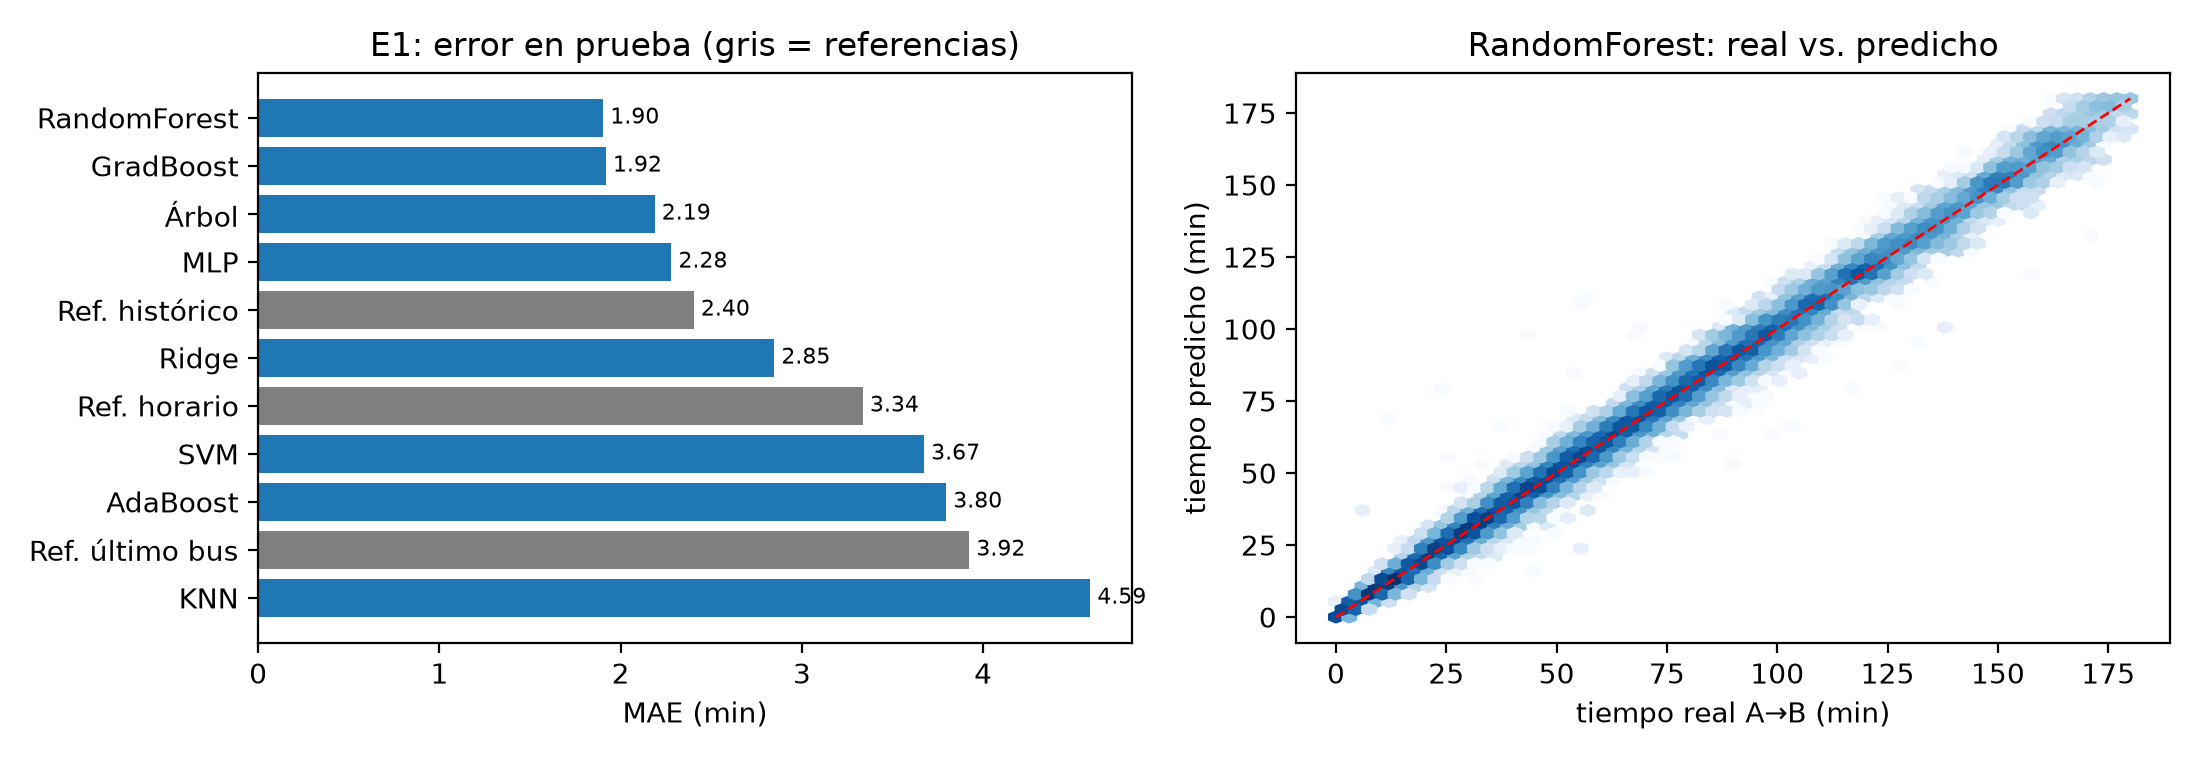
\includegraphics[width=0.85\textwidth]{exp1_comparacion.png}
\caption{E1. Izquierda: MAE en prueba (gris: referencias). Derecha: tiempo real frente al predicho por el mejor modelo (escala logarítmica de densidad).}
\label{fig:e1}
\end{figure*}

\textbf{E2: error según la distancia.} Como era de esperar, el error crece con $\Delta$ (Fig.~\ref{fig:e2} y Tabla~\ref{tab:delta}): el MAE del mejor modelo pasa de 0,85~min para el siguiente punto a 3,08~min para la vuelta completa. La ventaja sobre la mejor referencia también crece: es de 9,9\,\% en $\Delta = 1$ y supera el 15\,\% desde $\Delta = 4$, hasta 26,2\,\% en $\Delta = 17$. Para el siguiente punto el promedio histórico ya es difícil de superar, porque un tramo corto depende poco de lo que pase en el resto de la ruta; en trayectos largos, en cambio, el estado del bus y de los buses recientes permite anticipar retrasos que el promedio no ve.

\begin{table}[t]
\centering
\caption{E2: MAE (min) según la distancia $\Delta$ y mejora del mejor modelo}
\label{tab:delta}
\footnotesize
\setlength{\tabcolsep}{4pt}
\begin{tabular}{@{}rrrrrr@{}}
\toprule
$\Delta$ & Horario & Histórico & Último bus & Mejor & Mejora (\%) \\
\midrule
1 & 1,52 & 0,95 & 1,19 & 0,85 & 9,9 \\
2 & 1,98 & 1,46 & 1,89 & 1,28 & 12,1 \\
3 & 2,49 & 1,84 & 2,47 & 1,57 & 14,8 \\
5 & 3,25 & 2,37 & 3,42 & 1,95 & 17,7 \\
8 & 3,63 & 2,89 & 4,52 & 2,18 & 24,5 \\
12 & 5,25 & 3,50 & 6,88 & 2,55 & 27,0 \\
17 & 5,98 & 4,17 & 9,71 & 3,08 & 26,2 \\
\bottomrule
\end{tabular}
\end{table}

\begin{figure*}[t]
\centering
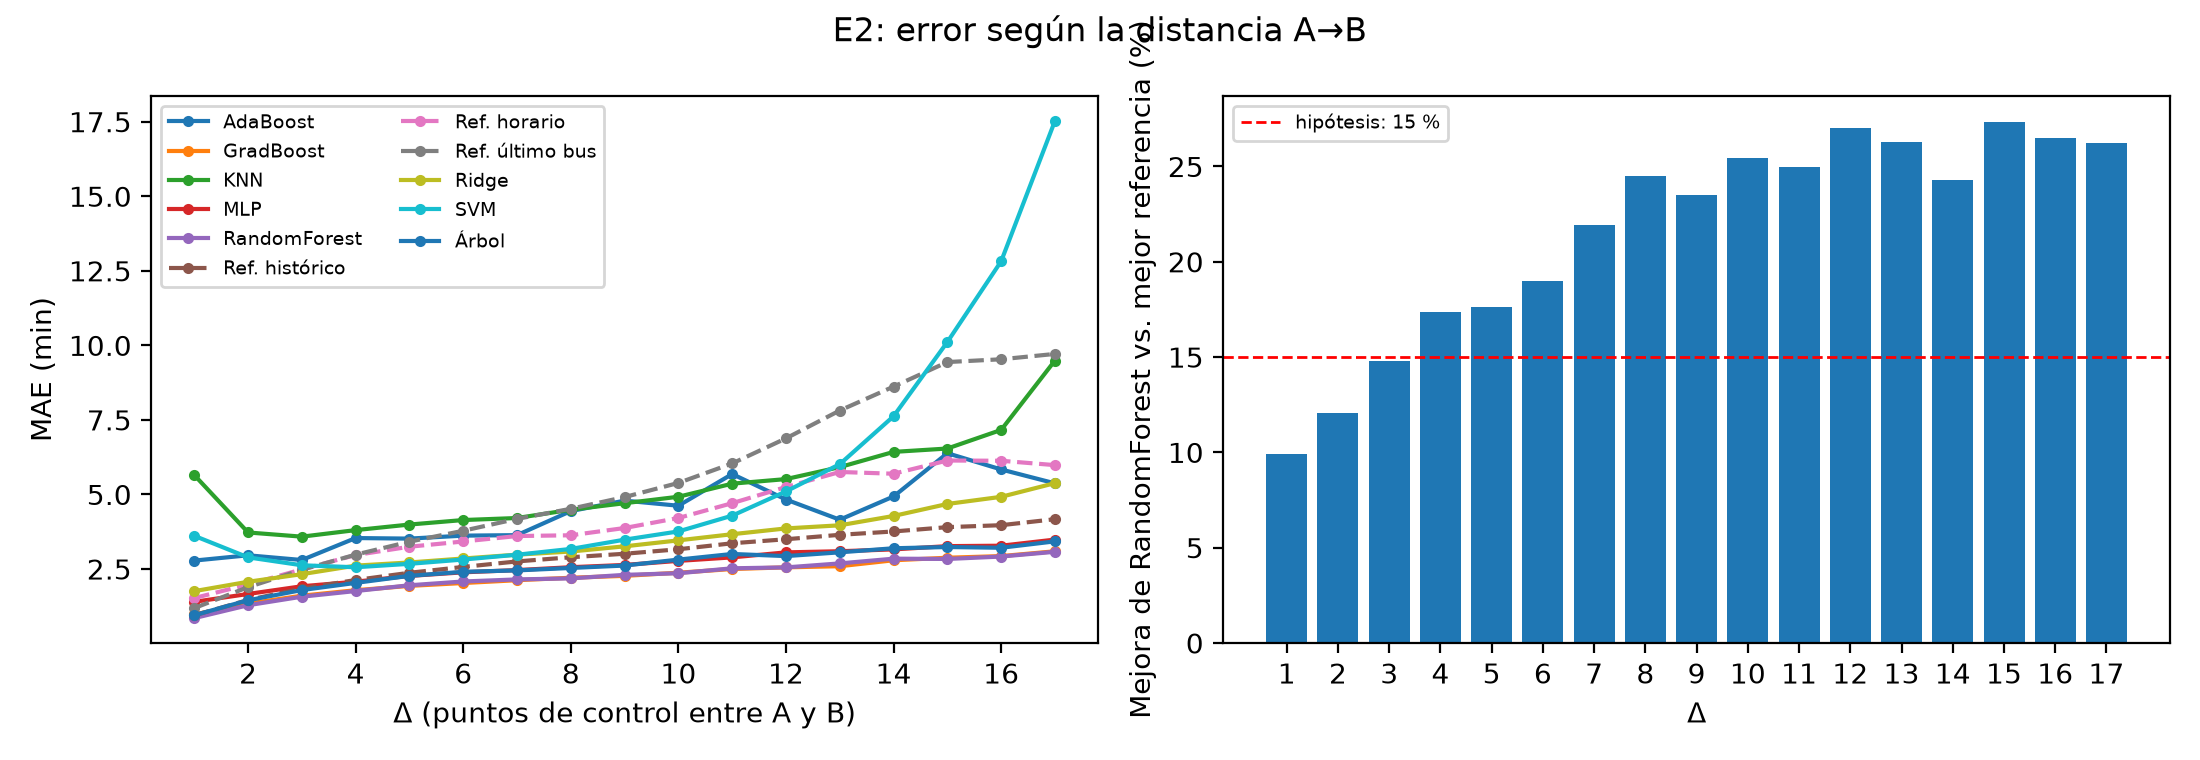
\includegraphics[width=0.85\textwidth]{exp2_horizonte.png}
\caption{E2. Izquierda: MAE por distancia $\Delta$ para todos los modelos. Derecha: mejora del mejor modelo frente a la mejor referencia en cada $\Delta$; la línea roja marca el 15\,\% de la hipótesis.}
\label{fig:e2}
\end{figure*}

\begin{figure*}[t]
\centering
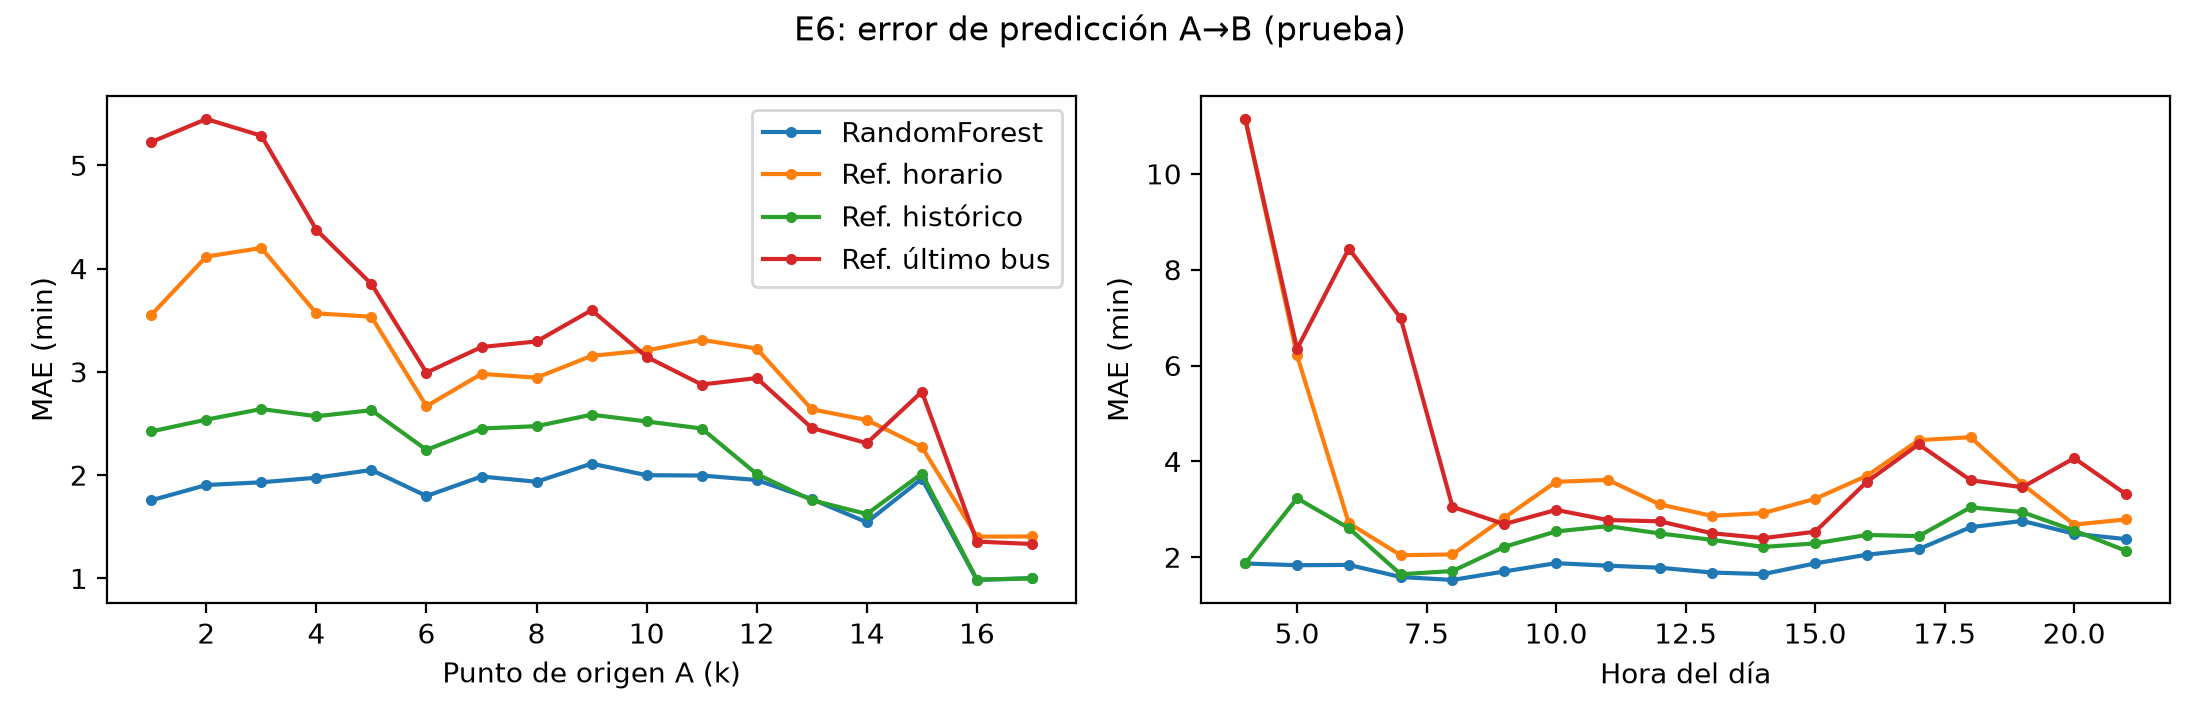
\includegraphics[width=0.85\textwidth]{exp6_errores.png}
\caption{E6. MAE en prueba por punto de origen (izquierda) y por hora del día (derecha) para el mejor modelo y las referencias.}
\label{fig:e6}
\end{figure*}

\begin{figure*}[t]
\centering
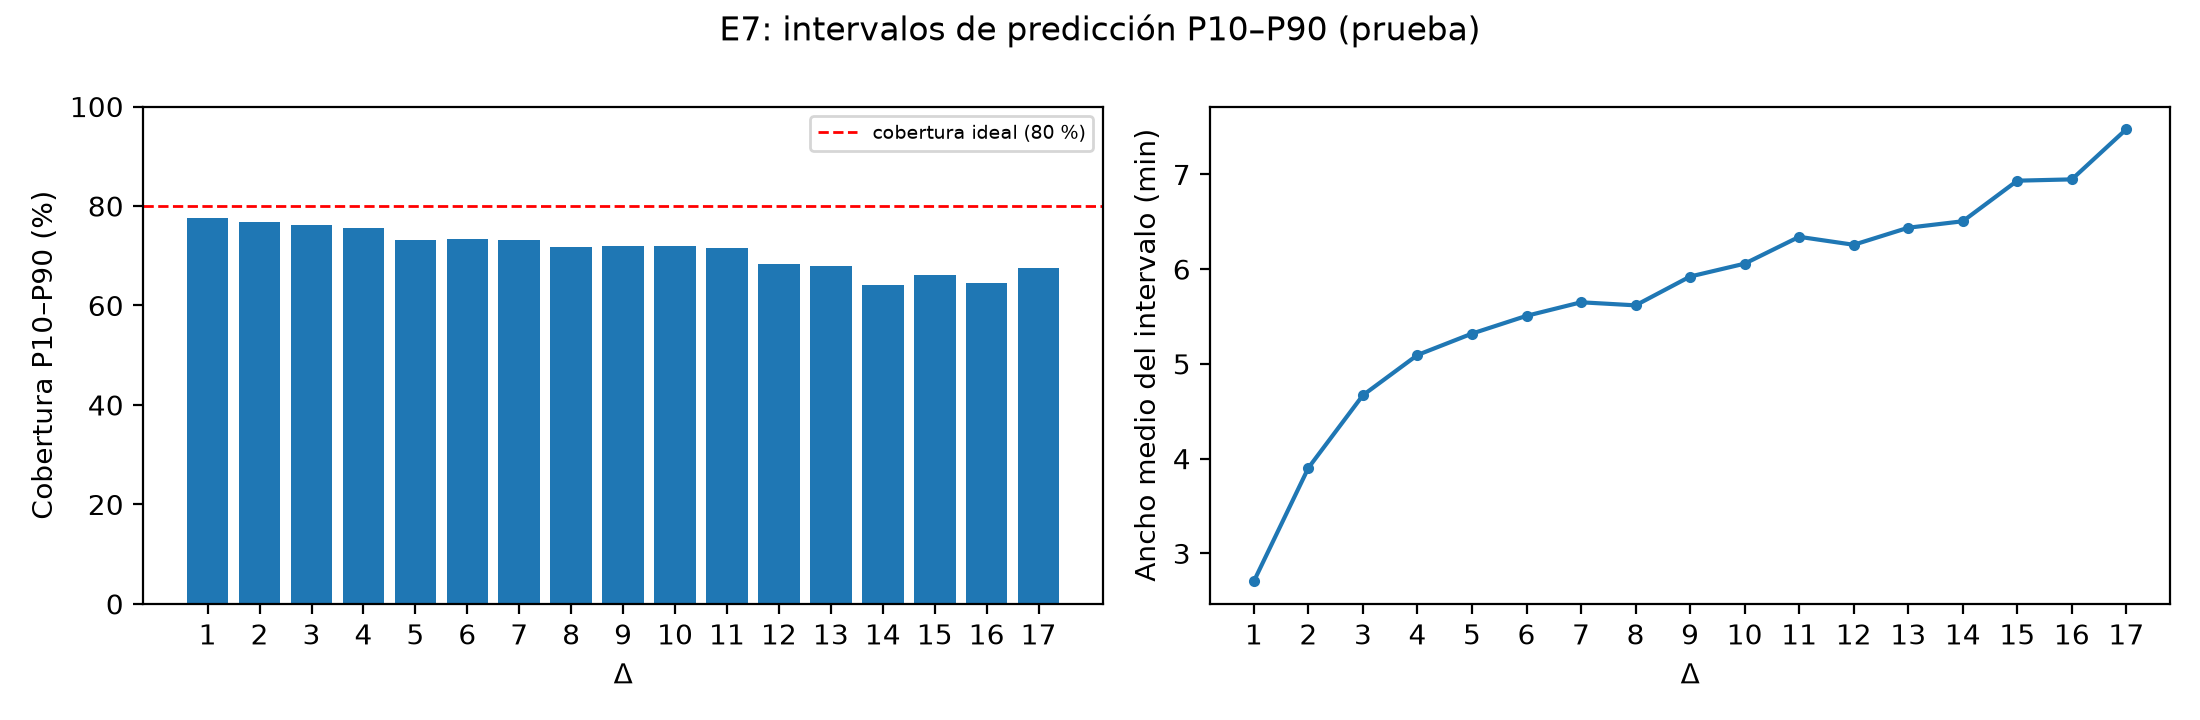
\includegraphics[width=0.85\textwidth]{exp7_intervalos.png}
\caption{E7. Cobertura del intervalo P10--P90 (izquierda; ideal 80\,\%) y ancho medio del intervalo (derecha) según la distancia $\Delta$.}
\label{fig:e7}
\end{figure*}

\textbf{E3: ablación de variables.} La Tabla~\ref{tab:abl} muestra el MAE de Gradient Boosting al quitar cada grupo. Las variables más útiles son el estado del bus (quitarlas sube el MAE en 10,2\,\%) y los buses recientes (3,2\,\%); con solo las variables de contexto el error sube 5,8\,\%. El GPS (0,1\,\%) y la altitud (0,1\,\%) prácticamente no cambian el error, porque sus efectos ya están recogidos en la duración de los tramos y en el origen. El clima, en cambio, \emph{empeora} el modelo: sin él, el MAE baja 3,7\,\% (1,85~min). Una explicación plausible es que, con solo 27 días de datos, cada combinación de valores climáticos corresponde prácticamente a un único día, de modo que el modelo puede usar el clima para memorizar días concretos del entrenamiento en lugar de aprender un efecto generalizable. La resolución del reanálisis (dos celdas para toda la ruta) y el hecho de que el efecto de la lluvia ya se refleja en los buses recientes contribuyen también a este resultado negativo.

\begin{table}[t]
\centering
\caption{E3: ablación por grupos de variables (Gradient Boosting)}
\label{tab:abl}
\footnotesize
\begin{tabular}{@{}lrrr@{}}
\toprule
Variables & N.\,º & MAE (min) & Cambio (\%) \\
\midrule
todas & 25 & 1,919 & -- \\
sin buses recientes & 22 & 1,980 & +3,2 \\
sin GPS & 21 & 1,920 & +0,1 \\
sin clima & 19 & 1,848 & -3,7 \\
sin altitud & 23 & 1,920 & +0,1 \\
sin estado del bus i & 20 & 2,115 & +10,2 \\
solo contexto & 5 & 2,031 & +5,8 \\
\bottomrule
\end{tabular}
\end{table}

\textbf{E4: PCA.} Conservar el 95\,\% de la varianza reduce las dimensiones de forma importante y acelera la predicción, pero no mejora el error de $k$NN ni de SVM (Tabla~\ref{tab:pca}): estos modelos siguen lejos de los ensambles, lo que indica que su limitación no es la dimensión sino la forma de la relación entre las variables y el tiempo de viaje.

\begin{table}[t]
\centering
\caption{E4: efecto de PCA en $k$NN y SVM}
\label{tab:pca}
\footnotesize
\begin{tabular}{@{}llrrr@{}}
\toprule
Modelo & PCA & Dimensiones & MAE (min) & Predicción (s) \\
\midrule
$k$NN & no & 70 & 4,59 & 31,9 \\
$k$NN & sí & 20 & 4,62 & 23,9 \\
SVM (RBF) & no & 70 & 3,67 & 112,3 \\
SVM (RBF) & sí & 20 & 3,98 & 87,7 \\
\bottomrule
\end{tabular}
\end{table}

\textbf{E5: hiperparámetros y costo.} La Tabla~\ref{tab:cost} muestra el rango del MAE de validación entre las combinaciones probadas y los tiempos del modelo final. Gradient Boosting y Ridge son poco sensibles a sus hiperparámetros, Random Forest y MLP lo son moderadamente, y SVM es muy sensible: su MAE de validación va de 4 a 25~min según $C$ y $\gamma$; AdaBoost y el árbol de decisión también varían bastante. En costo, Random Forest es por mucho el más lento de entrenar; Gradient Boosting ofrece casi el mismo error en una fracción del tiempo, por lo que es la opción más práctica para la demostración.

\begin{table}[t]
\centering
\caption{E5: rango del MAE de validación y costo del modelo final}
\label{tab:cost}
\footnotesize
\begin{tabular}{@{}lrrr@{}}
\toprule
Modelo & MAE val. (min) & Entren. (s) & Predicción (s) \\
\midrule
Random Forest & 2,43--2,58 & 4\,202 & 1,6 \\
Gradient Boosting & 2,45--2,50 & 58 & 5,4 \\
Árbol de decisión & 2,76--3,71 & 10 & 0,2 \\
MLP & 2,99--3,30 & 32 & 0,3 \\
Ridge & 3,48--3,49 & 2 & 0,1 \\
SVM (RBF) & 4,07--24,63 & 9 & 200,8 \\
AdaBoost & 4,12--5,58 & 161 & 4,3 \\
$k$NN & 5,52--5,92 & 0 & 26,6 \\
\bottomrule
\end{tabular}
\end{table}

\textbf{E6: análisis de errores y significancia.} El error del mejor modelo es menor que el de las tres referencias en casi todos los puntos de origen y horas (Fig.~\ref{fig:e6}). Las excepciones son los orígenes 16 y 17, cuyos trayectos son cortos y donde el modelo iguala al histórico, y las últimas horas de servicio (20:00--21:00), con pocos datos, donde el histórico es ligeramente mejor. El error crece en la tarde, cuando el tráfico es más variable, mientras que el horario y el último bus fallan sobre todo en la madrugada. La prueba de Wilcoxon sobre 918 bloques confirma que la mejora es estadísticamente significativa frente a cada referencia (Tabla~\ref{tab:w}).

\begin{table}[t]
\centering
\caption{E6: prueba de Wilcoxon (MAE por bloque día $\times$ origen $\times$ $\Delta$)}
\label{tab:w}
\footnotesize
\begin{tabular}{@{}lrrr@{}}
\toprule
Referencia & MAE ref. (min) & Mejora & $p$ \\
\midrule
Ref. horario & 3,50 & 43,9\,\% & $<10^{-10}$ \\
Ref. histórico & 2,51 & 21,7\,\% & $<10^{-10}$ \\
Ref. último bus & 4,03 & 51,3\,\% & $<10^{-10}$ \\
\bottomrule
\end{tabular}
\end{table}

\textbf{E7: intervalos de predicción.} El intervalo P10--P90 de la regresión cuantílica contiene al valor real en el 73,5\,\% de los casos de prueba, frente al 80\,\% ideal; el 14,7\,\% queda por debajo del P10 y el 11,8\,\% por encima del P90. La cobertura disminuye con la distancia, de 78\,\% a 64\,\% (Fig.~\ref{fig:e7}), y el ancho medio del intervalo crece de 2,7~min para el siguiente punto a 7,5~min para la vuelta completa (5,1~min en promedio). La mediana (P50) tiene un MAE de 1,90~min, similar al de la predicción puntual. Los intervalos son, por tanto, algo estrechos, sobre todo para trayectos largos: los cuantiles aprendidos no cubren del todo la variabilidad de la semana de prueba. Aun así, el rango es útil para la demostración si se comunica como orientativo, y puede calibrarse (ver trabajos futuros).

\textbf{Limitaciones.} Los datos cubren un solo mes y una sola ruta, por lo que no capturan la estacionalidad ni la temporada alta turística; la semana de prueba es corta (seis días), y las predicciones se limitan a los 18 puntos de control. Por costo, SVM, $k$NN, AdaBoost y MLP se entrenaron con submuestras, lo que puede subestimar su desempeño. La ablación (E3) se midió sobre el conjunto de prueba; por ello, la recomendación de retirar el clima debe confirmarse en validación antes de fijar el modelo final, para no seleccionar variables con los datos de prueba. Por último, las 88 anomalías detectadas por Isolation Forest (0,1\,\% de los pasos) se excluyen en todos los días, incluida la semana de prueba, lo que puede reducir ligeramente el error reportado.

% =====================================================================
\section{Conclusión}
Un modelo de regresión entrenado con los registros de puntos de control y GPS estima el tiempo de llegada entre dos puntos cualesquiera de la ruta con un MAE de 1,90~min, 20,8\,\% menor que el mejor método sin aprendizaje, lo que confirma la hipótesis. La ventaja crece con la distancia entre los puntos y proviene sobre todo del estado del bus y de los buses que acaban de recorrer el trayecto; el clima de reanálisis no aporta y la altitud y el GPS casi no cambian el error. Gradient Boosting logra prácticamente el mismo error que Random Forest con un costo mucho menor, y su versión cuantílica entrega un rango de llegada con una cobertura de 73,5\,\%, algo menor que el 80\,\% nominal.

% =====================================================================
\section{Sugerencias de trabajos futuros}
\begin{itemize}
\item Usar el modelo sin las variables de clima, que en este estudio empeoran el error, o incorporar lluvia medida en estaciones de la ruta.
\item Calibrar los intervalos (por ejemplo, con predicción conforme) para acercar la cobertura al 80\,\% en todas las distancias.
\item Estimar la llegada desde cualquier posición GPS del bus, no solo desde los puntos de control.
\item Ampliar el estudio a más meses y rutas, y probar modelos secuenciales sobre la serie de tramos de cada vuelta.
\end{itemize}

% =====================================================================
\section{Implicancias éticas}
Los datos GPS identifican vehículos e, indirectamente, a sus conductores. Las predicciones podrían usarse para sancionar a conductores por retrasos causados por el tráfico; por eso se recomienda usar el modelo para informar a los usuarios y planificar horarios, no para sanciones individuales, y anonimizar el identificador del vehículo, que además puede introducir sesgos contra ciertos conductores. Un tiempo de llegada mostrado con exceso de confianza puede hacer que un pasajero pierda su bus, por lo que conviene presentar siempre el rango P10--P90. Finalmente, el acceso a los datos de ubicación debe restringirse para proteger la privacidad de conductores y pasajeros.

% =====================================================================
\section{Repositorio del trabajo}
El código, las tablas de resultados y las figuras están en \url{https://github.com/Alfredo123255/prediccion-amontonamiento-buses-cusco}. El cuaderno \texttt{Experimentacion.ipynb} reproduce todos los resultados a partir de los archivos originales.

% =====================================================================
\section{Declaración de contribución}
\begin{itemize}
\item Divano Estefano Perez Nina: estructura inicial del repositorio, preprocesamiento de los datos de puntos de control y GPS, integración de los datos de clima y altitud, implementación de los experimentos E1--E7 en el cuaderno y redacción del borrador del paper del Entregable~2.
\item Ángel Fredy Cerdan Cigüeñas: análisis exploratorio de los datos y validación de los resultados experimentales, y revisión y redacción de secciones del paper.
\item Alfredo Ernesto Sanchez Tuesta: reformulación del problema como predicción del tiempo de llegada de A a B con un único modelo, definición de la hipótesis y de las métricas de evaluación, redacción del Entregable~1 con la revisión de trabajos relacionados, y revisión y corrección del paper del Entregable~2.
\item Renzo Kei Shimabukuro Kohatsu: contribuyó en la revisión de la metodología y el análisis de los resultados experimentales, especialmente en la interpretación de las métricas de evaluación, la comparación del rendimiento de los modelos y la identificación de sus limitaciones. Asimismo, apoyó en la revisión y redacción del informe final.
\end{itemize}

\textbf{Uso de inteligencia artificial generativa.} Se utilizó un asistente de IA generativa (Claude, de Anthropic) como apoyo para el análisis exploratorio, la programación del cuaderno y la redacción de borradores; la búsqueda bibliográfica se apoyó en Scopus AI. Los integrantes revisaron y validaron todo el contenido. Los registros de las interacciones están disponibles si el docente los solicita.

% =====================================================================
\begin{thebibliography}{99}
\footnotesize

\bibitem{concha2018}
C.~A. Concha~Vásquez, ``La lucha por la ciudad: controversias en el proceso de formulación del Plan Cusco al 2025 -- Movilidad y Espacio Público en una Ciudad Patrimonio (Cusco 2014-2018),'' \emph{Politai: Revista de Ciencia Política}, vol.~9, no.~16, pp.~141--176, 2018, doi: 10.18800/politai.201801.005.

\bibitem{delgado2021}
S.~Delgado y V.~Bellota, ``Calidad en el servicio de transporte público urbano en la ciudad del Cusco -- 2018,'' \emph{Revista Yachay}, vol.~10, no.~1, pp.~506--510, 2021, doi: 10.36881/yachay.v10i01.275.

\bibitem{chien2002}
S.~I.-J. Chien, Y.~Ding y C.~Wei, ``Dynamic bus arrival time prediction with artificial neural networks,'' \emph{J. Transp. Eng.}, vol.~128, no.~5, pp.~429--438, 2002, doi: 10.1061/(ASCE)0733-947X(2002)128:5(429).

\bibitem{bin2006}
B.~Yu, Z.~Yang y B.~Yao, ``Bus arrival time prediction using support vector machines,'' \emph{J. Intell. Transp. Syst.}, vol.~10, no.~4, pp.~151--158, 2006, doi: 10.1080/15472450600981009.

\bibitem{yu2011}
B.~Yu, W.~H.~K. Lam y M.~L. Tam, ``Bus arrival time prediction at bus stop with multiple routes,'' \emph{Transp. Res. Part C}, vol.~19, no.~6, pp.~1157--1170, 2011, doi: 10.1016/j.trc.2011.01.003.

\bibitem{petersen2019}
N.~C. Petersen, F.~Rodrigues y F.~C. Pereira, ``Multi-output bus travel time prediction with convolutional LSTM neural network,'' \emph{Expert Syst. Appl.}, vol.~120, pp.~426--435, 2019.

\bibitem{rodriguez2022}
H.~Rodríguez-Deniz y M.~Villani, ``Robust real-time delay predictions in a network of high-frequency urban buses,'' \emph{IEEE Trans. Intell. Transp. Syst.}, 2022, arXiv: 2106.13576.

\bibitem{reich2019}
T.~Reich, M.~Budka, D.~Robbins y D.~Hulbert, ``Survey of ETA prediction methods in public transport networks,'' arXiv: 1904.05037, 2019.

\bibitem{petersen2021}
N.~C. Petersen, A.~Parslov y F.~Rodrigues, ``Short-term bus travel time prediction for transfer synchronization with intelligent uncertainty handling,'' arXiv: 2104.06819, 2021.

\bibitem{koenker1978}
R.~Koenker y G.~Bassett, ``Regression quantiles,'' \emph{Econometrica}, vol.~46, no.~1, pp.~33--50, 1978.

\bibitem{friedman2001}
J.~H. Friedman, ``Greedy function approximation: A gradient boosting machine,'' \emph{Ann. Statist.}, vol.~29, no.~5, pp.~1189--1232, 2001.

\bibitem{mazloumi2010}
E.~Mazloumi, G.~Currie y G.~Rose, ``Using GPS data to gain insight into public transport travel time variability,'' \emph{J. Transp. Eng.}, vol.~136, no.~7, pp.~623--631, 2010, doi: 10.1061/(ASCE)TE.1943-5436.0000126.

\bibitem{liu2008}
F.~T. Liu, K.~M. Ting y Z.-H. Zhou, ``Isolation forest,'' en \emph{Proc. IEEE ICDM}, 2008, pp.~413--422.

\bibitem{tsapakis2013}
I.~Tsapakis, T.~Cheng y A.~Bolbol, ``Impact of weather conditions on macroscopic urban travel times,'' \emph{J. Transp. Geogr.}, vol.~28, pp.~204--211, 2013.

\bibitem{hersbach2020}
H.~Hersbach \emph{et~al.}, ``The ERA5 global reanalysis,'' \emph{Q. J. R. Meteorol. Soc.}, vol.~146, no.~730, pp.~1999--2049, 2020.

\bibitem{pedregosa2011}
F.~Pedregosa \emph{et~al.}, ``Scikit-learn: Machine learning in Python,'' \emph{J. Mach. Learn. Res.}, vol.~12, pp.~2825--2830, 2011.

\bibitem{breiman2001}
L.~Breiman, ``Random forests,'' \emph{Mach. Learn.}, vol.~45, no.~1, pp.~5--32, 2001.

\bibitem{bergmeir2012}
C.~Bergmeir y J.~M. Benítez, ``On the use of cross-validation for time series predictor evaluation,'' \emph{Inf. Sci.}, vol.~191, pp.~192--213, 2012.

\bibitem{hyndman2006}
R.~J. Hyndman y A.~B. Koehler, ``Another look at measures of forecast accuracy,'' \emph{Int. J. Forecast.}, vol.~22, no.~4, pp.~679--688, 2006.

\bibitem{demsar2006}
J.~Demšar, ``Statistical comparisons of classifiers over multiple data sets,'' \emph{J. Mach. Learn. Res.}, vol.~7, pp.~1--30, 2006.

\end{thebibliography}

\end{document}
